\input{Header-Comp.tex}

\begin{document}

\begin{page}
\begin{tikzpicture}[yscale=1]

	\def\yMax{7.5}
	\def\yMaxp{\yMax-0.5}
	\def\xMax{7.5}
	\def\xMaxp{\xMax-0.5}
	\def\clkMax{0.4*\yMax}	
	\def\startMin{0.5*\yMax}

	%CURVA: CLK
	\draw[draw=orange, thick] (0,0) -| (0.1*\xMax,\clkMax) -| (0.3*\xMax,0) -| (0.6*\xMax,\clkMax) -| (0.8*\xMax,0) -- (\xMaxp,0);
	
	%CURVA: START
	\draw[draw=purple, thick] (0,\startMin) -| (0.3*\xMax,\yMaxp) -| (0.35*\xMax,\startMin) -| (0.8*\xMax,\yMaxp) -| (0.85*\xMax,\startMin) -- (\xMaxp,\startMin);
	
	%LABELS
	\draw 
		(0,1.5*\startMin) node[label=left:\tiny{\textcolor{purple}{$START$}}](){}
		(0,0.5*\clkMax) node[label=left:\tiny{\textcolor{orange}{$CLK_{SH}$}}](){}
		(0.2*\xMax,0) node[label=below:\tiny{\textcolor{orange}{$T_{SAMPLE}$}}](){}
		(0.45*\xMax,0) node[label=below:\tiny{\textcolor{orange}{$T_{HOLD}$}}](){}
		(0.325*\xMax,1.1*\yMax) node[label=below:\tiny{\textcolor{purple}{$T_{WS}$}}](){}
	;
	
	%DASHED
	\draw[dashed]
		(0.3*\xMax,0) -- (0.3*\xMax,\yMax)
		(0.35*\xMax,0) -- (0.35*\xMax,\yMax)
		(0.6*\xMax,0) -- (0.6*\xMax,\yMax)
		(0.8*\xMax,0) -- (0.8*\xMax,\yMax)
	;	

	%EJES
	\draw[->][draw=black, very thick] (0,0) -- (0,\yMax);
	\draw[->][draw=black, very thick] (0,0) -- (\xMax,0);
	\draw (0,0) ++ (0,\yMax) node[label=right:{\textcolor{black}{$V$}}](){};
	\draw (0,0) ++ (\xMax,0) node[label=right:{\textcolor{black}{$t$}}](){};
	
\end{tikzpicture}
\end{page}

\newcommand{\pulse}[3] % #1 = length #2 = duty cicle #3 = height 
{
	|- ++ (#2*#1, #3) |- ++ ($ (#1, -1*#3) !#2! (0,-1*#3) $)
}

\begin{page}
\begin{tikzpicture}[yscale=1]

	\def\yMax{7.5}
	\def\yMaxp{7}
	\def\xMax{7.5}
	\def\xMaxp{7}
	\def\rowHeigth{\yMaxp*0.25}
	\def\rowForPulse{\rowHeigth*0.8}
	
	%PULSO: AND (A, B, C)
	\draw[draw=red, thick] (0,0) \pulse{0.5*\xMaxp}{0.125}{\rowForPulse} \pulse{0.5*\xMaxp}{0.125}{\rowForPulse} ++ (1,0.5) node[label=right:{\textcolor{black}{$A\&B\&C = f_{conv}$}}](){};
	
	%PULSO: C
	\draw[draw=magenta, thick] (0,\rowHeigth) \pulse{0.125*\xMaxp}{0.5}{\rowForPulse} \pulse{0.125*\xMaxp}{0.5}{\rowForPulse} \pulse{0.125*\xMaxp}{0.5}{\rowForPulse} \pulse{0.125*\xMaxp}{0.5}{\rowForPulse}  \pulse{0.125*\xMaxp}{0.5}{\rowForPulse} \pulse{0.125*\xMaxp}{0.5}{\rowForPulse} \pulse{0.125*\xMaxp}{0.5}{\rowForPulse} \pulse{0.125*\xMaxp}{0.5}{\rowForPulse} ++ (1,0.5) node[label=right:{\textcolor{black}{$\frac{f_{CLK}}{88} = C$}}](){};
	
	%PULSO: B
	\draw[draw=violet, thick] (0, 2*\rowHeigth) \pulse{0.5*\xMaxp}{0.5}{\rowForPulse} \pulse{0.5*\xMaxp}{0.5}{\rowForPulse} ++ (1,0.5) node[label=right:{\textcolor{black}{$\frac{f_{CLK}}{44} = B$}}](){};

	%PULSO: A
	\draw[draw=blue, thick] (0, 3*\rowHeigth) \pulse{\xMaxp}{0.5}{\rowForPulse} ++ (1,0.75) node[label=right:{\textcolor{black}{$\frac{f_{CLK}}{22} = A$}}](){};

	%EJES
	\draw[->][draw=black, very thick] (0,0) -- (0,\yMax);
	\draw[->][draw=black, very thick] (0,0) -- (\xMax,0);
	\draw (0,0) ++ (0,\yMax) node[label=right:{\textcolor{black}{$V$}}](){};
	\draw (0,0) ++ (\xMax,0) node[label=right:{\textcolor{black}{$t$}}](){};
	
\end{tikzpicture}
\end{page}


\begin{page}
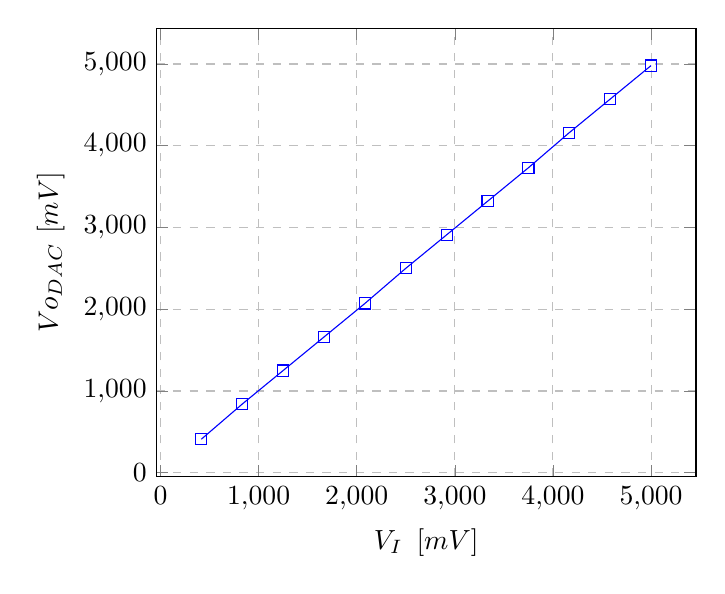
\begin{tikzpicture}
\begin{axis}[
%    title={Temperature dependence of CuSO$_4\cdot$5H$_2$O solubility},
    xlabel={$V_I \ \left[ mV \right]$},
    ylabel={$Vo_{DAC} \ [mV]$},
%    xmin=0, xmax=100,
%    ymin=0, ymax=120,
%    xtick={0,20,40,60,80,100},
%    ytick={0,20,40,60,80,100,120},
    legend pos=north west,
    xmajorgrids=true,
    ymajorgrids=true,
    grid style=dashed,
]

\addplot[
    color=blue,
    mark=square,
    ]
	coordinates { (416.666, 410.01)(833.333, 839.84)(1250, 1250)(1666.66,1660.15)(2083.33,2070.3)(2500,2500)(2916.66,2910.15)(3333.33,3320.31)(3750,3730.46)(4166.66,4160.15)(4583.33,4570.31)(5000,4980.46)    
    };
%    \legend{CuSO$_4\cdot$5H$_2$O}
\end{axis}
\end{tikzpicture}
\end{page}

\begin{page}
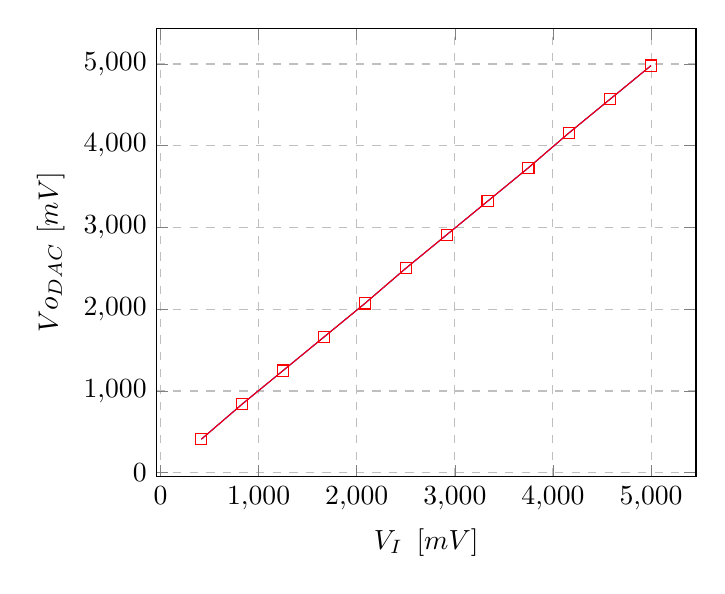
\begin{tikzpicture}
\begin{axis}[
%    title={Temperature dependence of CuSO$_4\cdot$5H$_2$O solubility},
    xlabel={$V_I \ \left[ mV \right]$},
    ylabel={$Vo_{DAC} \ [mV]$},
%    xmin=0, xmax=100,
%    ymin=0, ymax=120,
%    xtick={0,20,40,60,80,100},
%    ytick={0,20,40,60,80,100,120},
    legend pos=north west,
    xmajorgrids=true,
    ymajorgrids=true,
    grid style=dashed,
]

\addplot[
    color=blue,
    mark=square,
    ]
	coordinates { (416.666, 410.01)(833.333, 839.84)(1250, 1250)(1666.66,1660.15)(2083.33,2070.3)(2500,2500)(2916.66,2910.15)(3333.33,3320.31)(3750,3730.46)(4166.66,4160.15)(4583.33,4570.31)(5000,4980.46)    
    };
\addplot[
    color=red,
    mark=square,
    ]
	coordinates { (416.666, 410.01)(833.333, 839.84)(1250, 1250)(1666.66,1660.15)(2083.33,2070.3)(2500,2500)(2916.66,2910.15)(3333.33,3320.31)(3750,3730.46)(4166.66,4160.15)(4583.33,4570.31)(5000,4980.46)    
    };
%    \legend{CuSO$_4\cdot$5H$_2$O}
\end{axis}
\end{tikzpicture}
\end{page}

\begin{page}
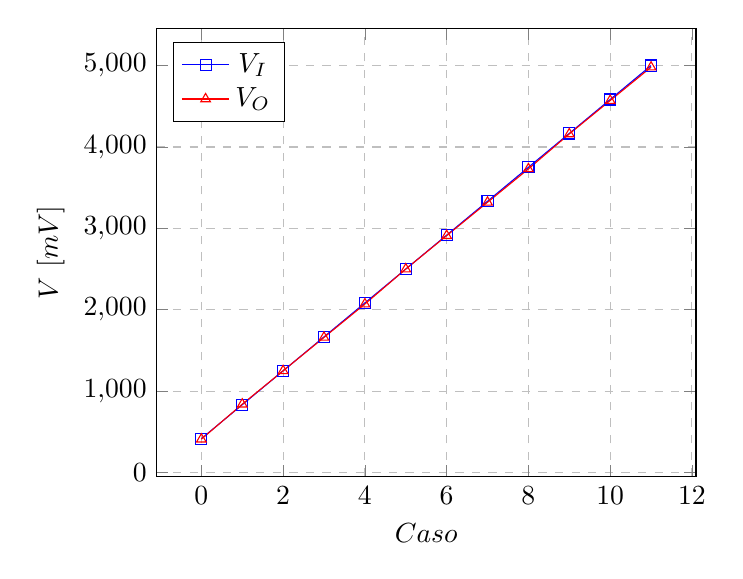
\begin{tikzpicture}

\begin{axis}[ xlabel={$Caso$}, ylabel={$V \ [mV]$}, legend pos=north west, xmajorgrids=true, ymajorgrids=true, grid style=dashed,]

\addplot[ color=blue, mark=square,]    
	coordinates { (0, 416.666)(1, 833.333)(2, 1250)(3, 1666.66)(4, 2083.33)(5, 2500)(6, 2916.66)(7, 3333.33)(8, 3750)(9, 4166.66)(10, 4583.330)(11, 5000)    
    };    

\addlegendentry{$V_I$}
    
\addplot[color=red, mark=triangle,]	
	coordinates { (0, 410.01)(1, 839.84)(2, 1250)(3, 1660.15)(4, 2070.3)(5, 2500)(6, 2910.15)(7, 3320.31)(8, 3730.46)(9, 4160.15)(10, 4570.31)(11, 4980.46)    
    };
    \addlegendentry{$V_O$}
    
\end{axis}
\end{tikzpicture}
\end{page}

\end{document}